\renewcommand{\figurename}{}
\mychapter{R305 Chaîne de transmission numérique (27h)}{cap:r305}
\lhead{R305 Chaîne de transmission numérique (27h)}

\vspace*{0.2cm}%
      \large
      \href{\@orientadorPagina}{\color{black}Enseignant\\Mr. Angel Abénia}\\%
\vspace*{0.5cm}%

Le module R305 a été abordé pendant la première période à l'IUT, son examen s'est déroulé sur la deuxième période pendant une heure. Ce module avait comme objectif la meilleure caractérisation des supports de transmission en étudiant de manière plus approfondie la transmission des signaux, donc leur étude.

\section{Caractérisation d'un canal de transmission}

Une mise en matière à ce module pourrait être les informations suivantes.
\begin{itemize}
  \item Pour communiquer, les appareils ont besoin d'avoir des informations à échanger, sinon ils n'auraient pas eu besoin d'avoir à communiquer.
  \item Les informations sont véhiculées par un signal, électromagnétique, optique, électrique ou hertzien.
  \item Un support, ou canal de transmission, est utilisé pour transmettre les signaux. Celui-ci est adapté selon la nature du support physique et le type de signal à transporter.
\end{itemize}

\begin{figure}[h]
    \centering
    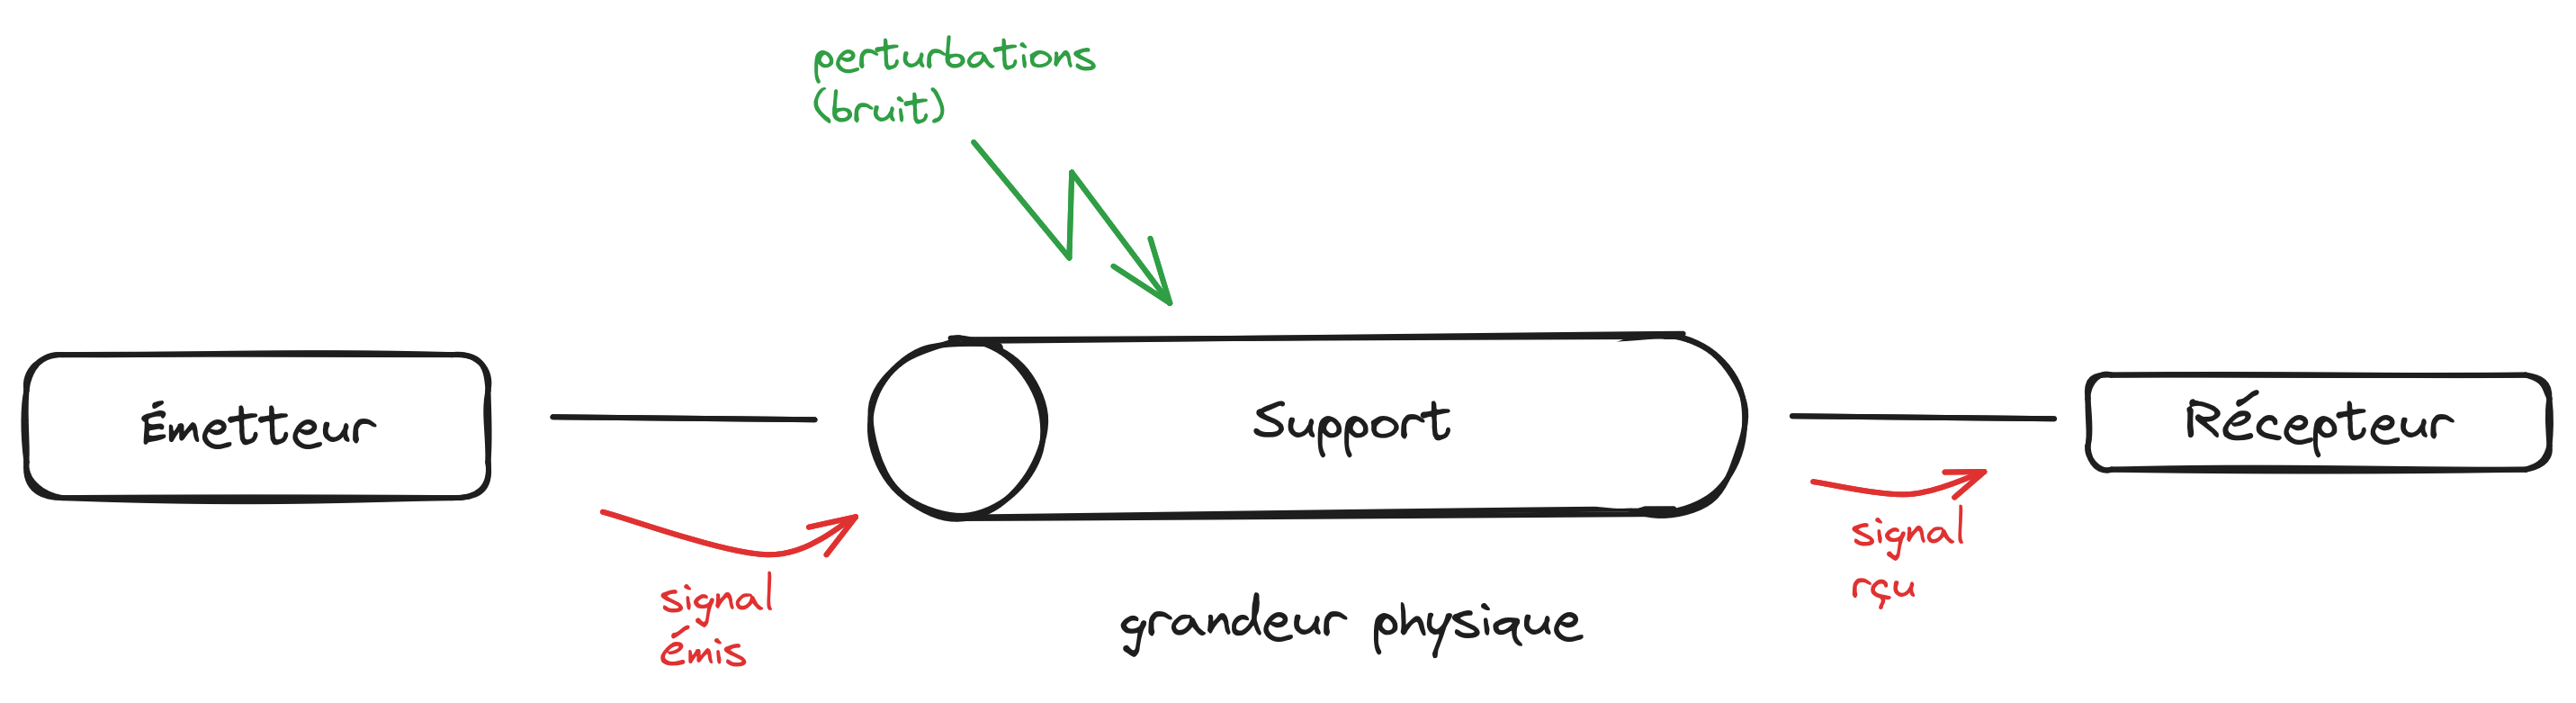
\includegraphics[width=1\linewidth]{imgs/support.png}
    \caption{Schéma représentatif d'un canal de transmission}
    \label{fig:canal}
\end{figure}

Un support de transmission admet une Bande passante \textbf{Bp}. Celle-ci est caractérisée par l'ensemble des fréquences que le canal permet de transporter. Ainsi que leur localisation dans l'espace des fréquences. Une bande passante admet donc une fréquence de début, une de fin, et une dernière centrale.
\\ \\
Bp de 100 Hz centrée sur 50 Hz. Soit Bp permet de transmettre toute fréquence dans l'intervale [0 Hz ; 100 Hz]
\\ \\
À leur dépassement à ses extrémités, le signal ne sera pas bien transmis; trop de dégradations seront appliquées pour les fréquences en dehors de la bande passante. Si nous pouvions avoir un canal de transmission parfait, avec aucune limite de bande passante et sans atténuation, alors le débit maximal théorique obtenable serait parfait aussi, outrepassant toute loi de la physique mais utile pour des calculs.
\\ \\
Ainsi, un canal de transmission avec une meilleure bande passante permet un meilleur débit binaire théorique : e.g. avec la fibre optique et une paire torsadée. Le signal "ne va pas plus vite", la vitesse de l'électricité dans un conducteur étant relativement proche de celle de la lumière dans du silice, mais la bande passante permise par le changement de support permet un meilleur débit, par la fibre moins d'atténuation, facilitant l'élargissement de la bande passante.
\\ \\
Dans la caractérisation de la chaîne de transmission du monde du numérique, nous avons rappelé le principe de liaison synchrone et asynchrone (synchronisation des horloges ou resynchronisation du front de décision à chaque information). Nous avons aussi revu le principe de débit binaire maximal théorique (brut), et celui dit "net" à l'utilisation - après toutes les informations nécessaires à la transmission des données ajoutées pour assurer sa transmission (dans les entêtes et queues des couches des protocoles).
\\ \\
Dans la caractérisation d'un signal, nous avons vu l'apparition des zones de décision pour différencier les états significatifs d'un signal. Pouvant se traduire par la plage de décision permise pour définir si l'on peut différencier un état significatif du signal (codant une information), pouvant laisser place à une zone d'incertitude. La place de décision doit toujours être inférieure au temps d'un état, sinon possibilité de confusion.

\begin{figure}[h]
    \centering
    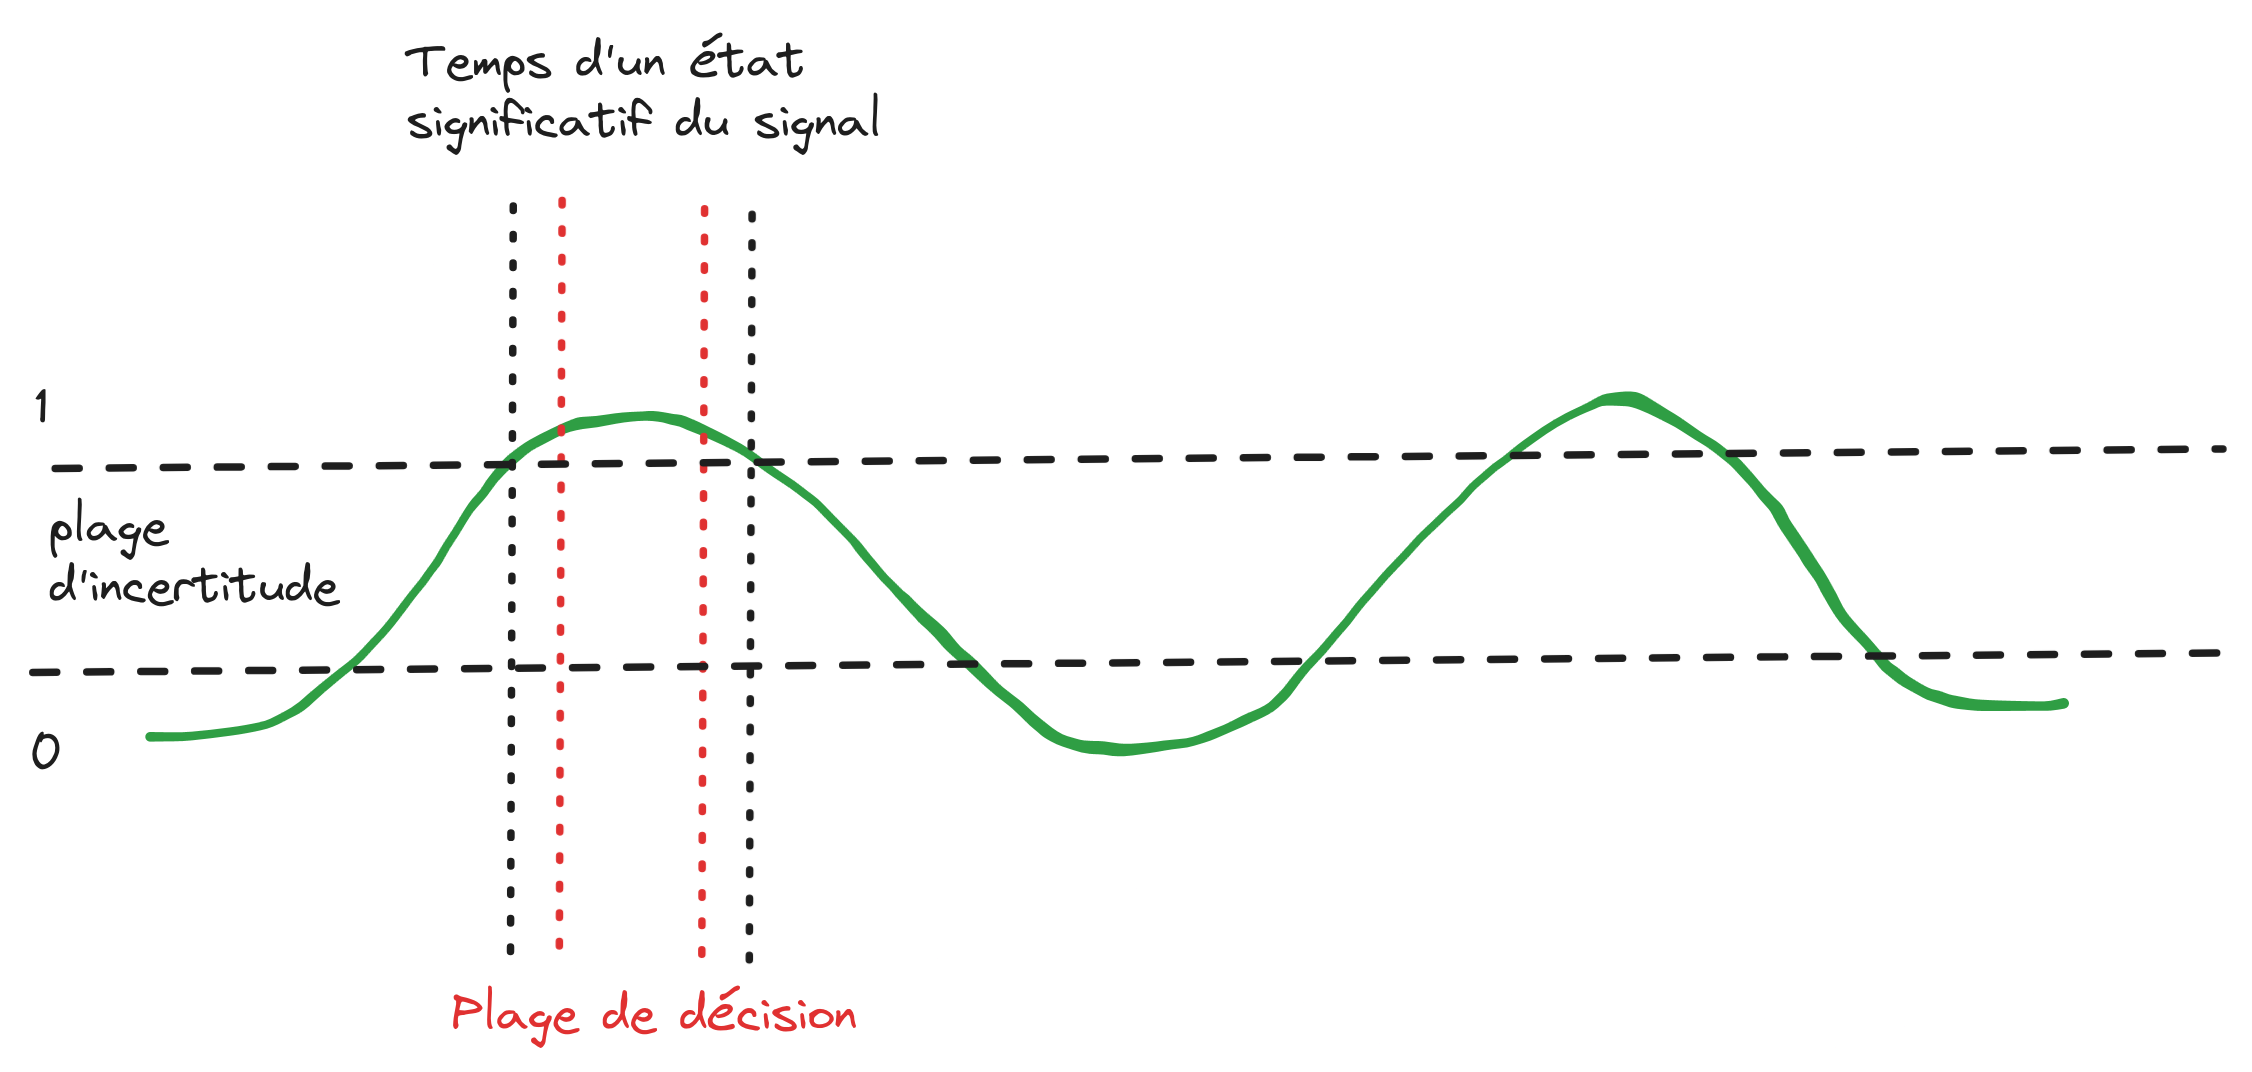
\includegraphics[width=1\linewidth]{imgs/td.png}
    \caption{Schéma représentatif de la décision d'un état pour une sinusoïde simple, ou "comment définir l'état d'un signal"}
    \label{fig:td}
\end{figure}

Par ce schéma, on peut en ressortir que si une plage de décision est trop large comparée au moment d'un symbole (état significatif d'un signal) : on peut confondre un état pour un autre. Il s'agit de l'interférance inter-symbole, ici représenté par deux états électriques +A -A (A pouvant être négatif). L'intérêt est de bien configurer les seuils de décisions (encadrement des valeurs du signal - plage d'incertitude) et les temps de décisions (plage de décision d'un moment).
\\ \\
Un autre moyen plus simple de mettre en évidence l'interférance inter-symbole est de diagramme de l'oeil. Dans celui-ci sont défini tous les passages possibles des états.

\begin{figure}[h]
    \centering
    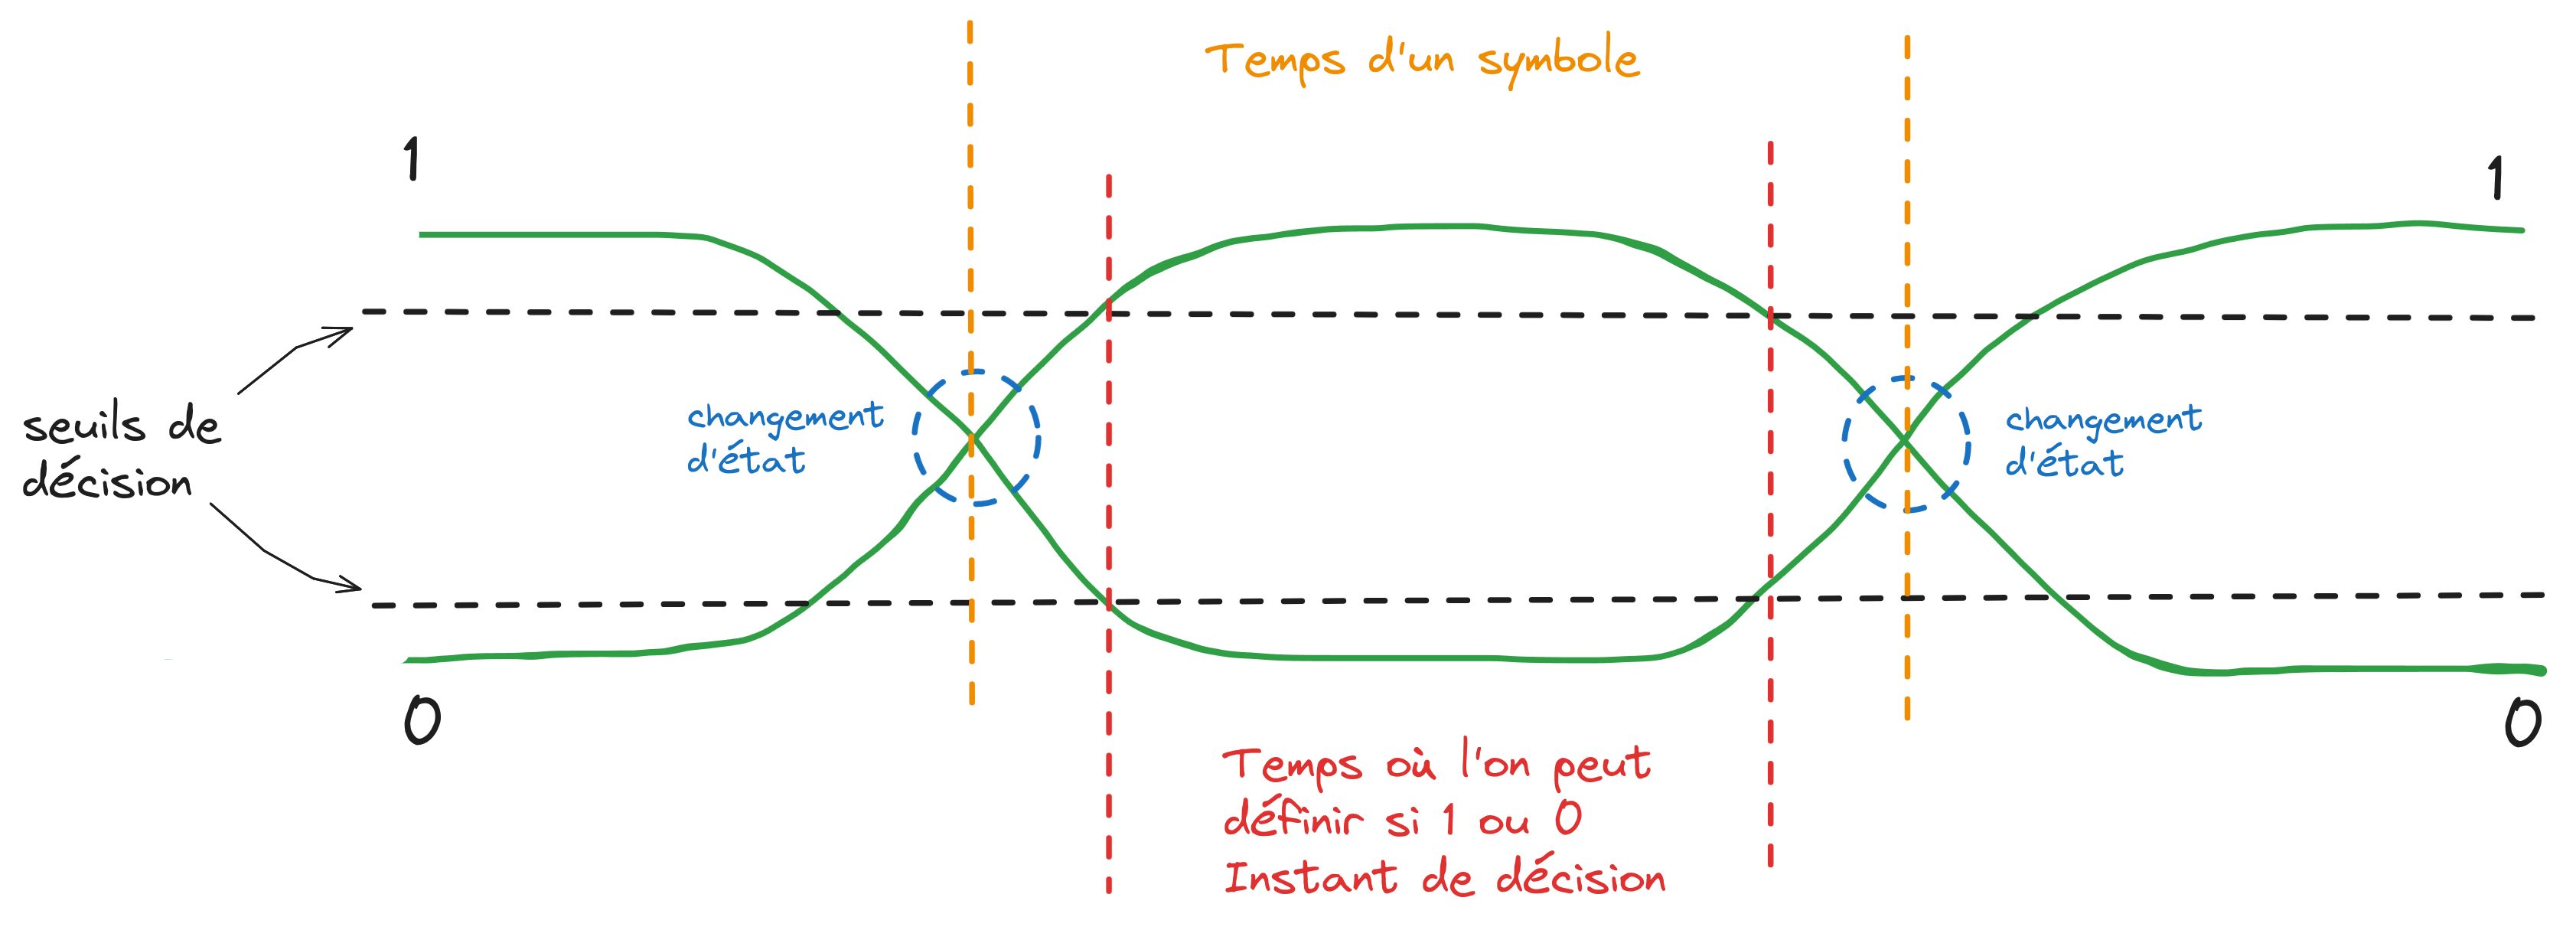
\includegraphics[width=1\linewidth]{imgs/seuils.png}
    \caption{Introduction au diagramme de l'oeil par identification des états d'un signal carré sans bruit (très fin)}
    \label{fig:seuils}
\end{figure}

Le temps où l'on peut définir si l'état est à 0 ou 1 ne peut être plus grand ou égale qu'à celui des symboles, sinon interférence inter-symbole. Le temps d'un symbole commence dès le changement du précédent état. Si l'instant de décision n'est pas correcte, deux choix pour atteindre les seuils si on ne peut pas les modifier : diminuer le débit pour faire rentrer le signal dans leur intervale, ou augmenter la bande passante - en changeant de canal de transmission.
%\\ \\
%Nous avons fait la différence entre le débit binaire brute théorique attégnable, et celui reçu après informations rajoutées aux données envoyées (destination dans un réseau, gestion de sessions, encapsulation de protocoles...) dans des entêtes et/ou des queues.
\\ \\
Nous pouvons changer le débit en conservant une bande passante correcte en jouant sur la valence du signal. En conservant la même fréquence, nous pouvons moduler le signal en amplitude ou en phase afin d'avoir davantage de symboles. La limite de cette pratique nous est donné par les travaux de Mr. Shanon que nous avons étudié, fixant que la valence se limite à ce que permet le rapport signal sur bruit, pour distinguer tous les états.
\\ \\
Nous avons aussi repris les travaux de Mr. Nyquist en intégrant ses critères pour définir la capacité d'un canal, soit sa bande passante maximale dans le domine théorique et physique. Nous avons notamment démontré la différence entre ces deux en travaux pratiques.
\\ \\
Si le débit binaire augmente, la bande passante aussi, sinon interférence entre les symboles. Pour contrer ceci soit augmenter la bande passante, soit réduire le débit, soit jouer sur les seuils et les instants de décision. D'autres états peuvent être introduits par modulation, à question que ceux-ci puissent être distingués, donc pas limités par le rapport entre le niveau de puissance du signal et celui du bruit.

\section{Fiabilisation d'une transmission}

La fiabilisation d'une transmission peut se caractériser par sa capacité à transmettre un message selon des circonstances données. Ainsi, des mécanismes de contrôle d'erreurs sont instaurés avec une demande de ré-émission par exemple. Le choix du type de transmission est aussi important, sa modulation. Dans cette partie nous avons abordé les codecs et nous avons étudié les types de modulation (manchester, NRZ...).
\\ \\
Certains types de modulations permettent une meilleur résistance au bruit, notamment ceux par phase vu diagramme de constellation. Chacun code le signal comme il le souhaite, le temps et les chercheurs sont par exemple passés du codage NRZ \textit{non-return-to-zero} à du PSK \textit{Phase-shift keying} ou du QAM \textit{quadrature amplitude modulation} toujours utilisés aujourd'hui. Leur largeur de spectre pour les mêmes informations envoyées changent aussi, pareil que pour son emplacement dans un spectre d'amplitude (lobe principal centré sur 0 Hz pour ceux qui ne modulent pas en fréquence...).

\section{Aboutissants du module}

Nous avons approfondi nos connaissance dans les supports de transmissions qui nous servent aujourd'hui. Nous pouvons les caractériser correctement pour montrer une infrastructure, nous pouvons les diagnostiquer dans nos domaines de compétences. Nous comprenons désormais comment circule un signal dans la "chaine du transmission du numérique", son histoire et son arrivée au monde moderne.